\documentclass{beamer}

\usepackage{amssymb}
\usepackage{amsmath}
\setcounter{tocdepth}{3}
\usepackage{graphicx}
\usepackage{cite}
\usepackage{bm}
% \usepackage[version=3]{mhchem}
\usepackage{import}
\usepackage{multirow}
\usepackage{hhline}
\usepackage{parcolumns}
\usepackage{caption}
\usepackage{subcaption}
\usepackage{longtable}
%\usepackage{natbib}
\usepackage{array}
\usepackage{verbatim}

%\usepackage[slovene]{babel}
\usepackage[utf8x]{inputenc}
\usepackage[T1]{fontenc}
%\usepackage[usenames,dvipsnames,svgnames,table]{xcolor}	
%\usepackage{lmodern}

\newcommand{\mx}[1]{\ensuremath{\textbf{#1}}}
\newcommand{\beq}{\begin{equation*}}
\newcommand{\eeq}{\end{equation*}}
\setbeamertemplate{footline}[frame number]

\begin{document}
  
\title[Crisis] % (optional, only for long titles)
{Practical examples of Time Series Data Visualizations}

\author[Author, Anders] % (optional, for multiple authors)
{Martin Stražar}
\institute{ Bioinformatics Laboratory, Faculty of Computer and Information Science, University of Ljubljana, Tržaška 25, 1000 Ljubljana, Slovenia  
}
\date[KPT 2004] % (optional)
{\today}

\maketitle

\begin{frame}
	\frametitle{Plotting time series data}
	\framesubtitle{Stack plot}
	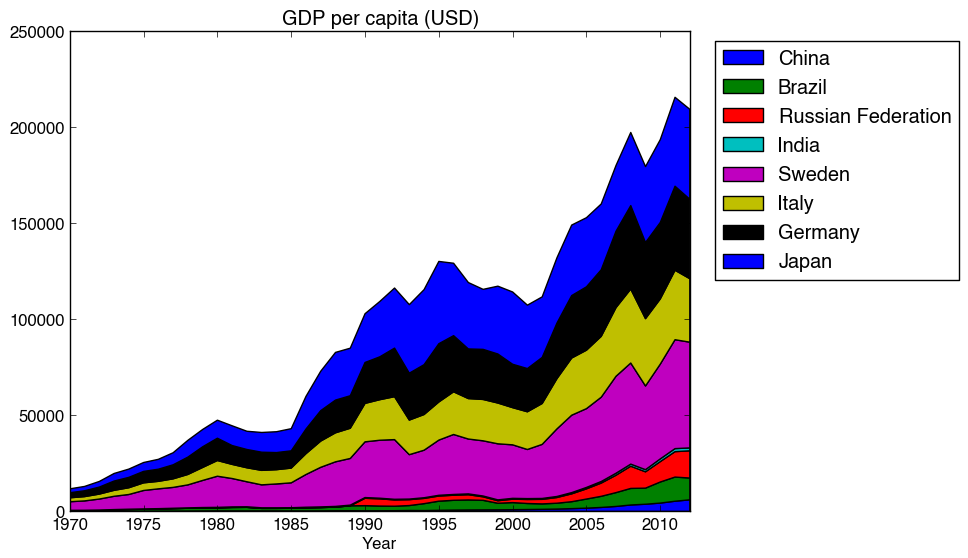
\includegraphics[scale=0.4]{../results/gdp.png}
\end{frame}

\begin{frame}
	\frametitle{Plotting time series data}
	\framesubtitle{Stack plot (normalized)}
	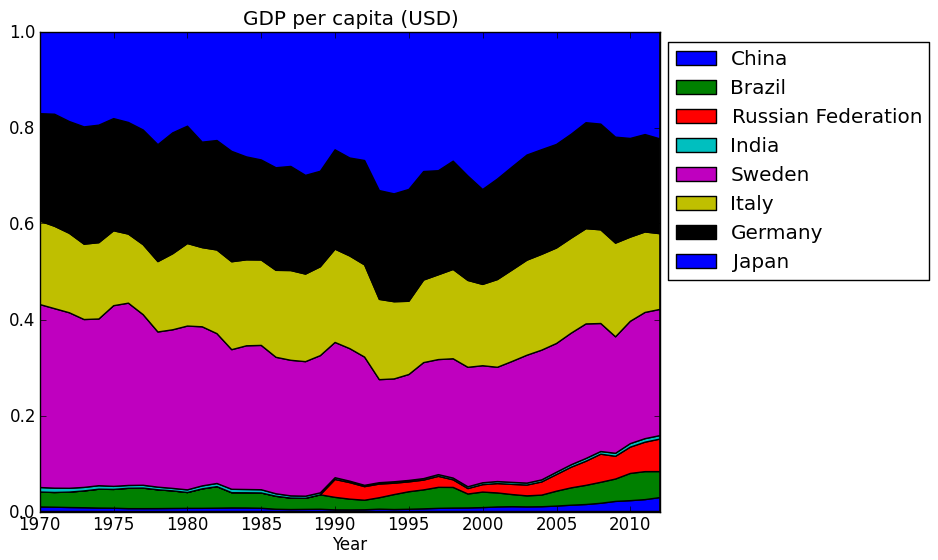
\includegraphics[scale=0.5]{../results/gdpn.png}
\end{frame}
 
 \begin{frame}
	\frametitle{Google trends}
	\url{http://www.google.com/trends/}
\end{frame} 

\begin{frame}
	\frametitle{Animation}
	\framesubtitle{Density of population in Ireland}
	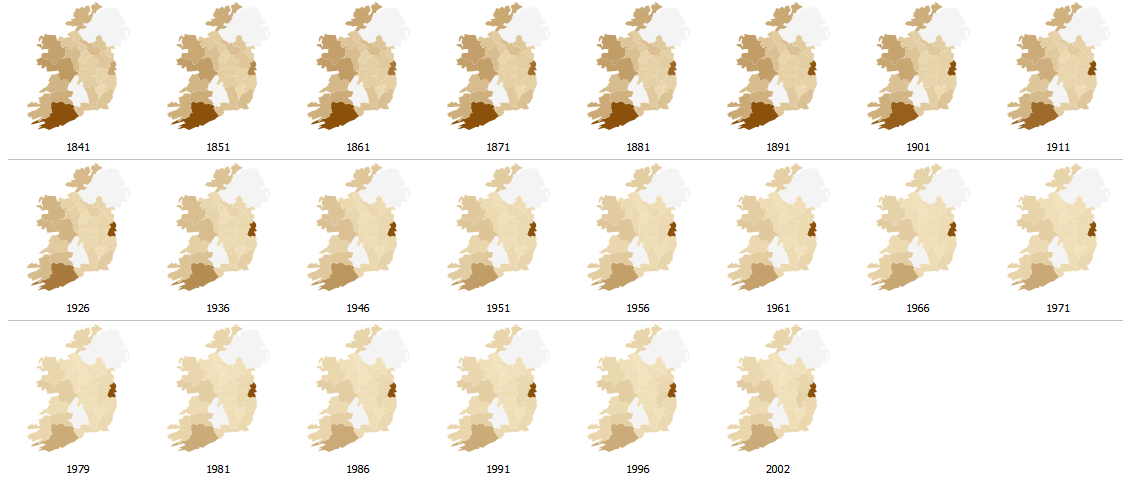
\includegraphics[scale=0.4]{../img/irci-v-dublin.png}
\end{frame} 

\begin{frame}
	\frametitle{Animation}
		GapMinder World
		\url{http://www.gapminder.org/downloads/}
\end{frame} 

\begin{frame}
	\frametitle{Animation}
	\framesubtitle{Proportion of citizen over 65 years}
	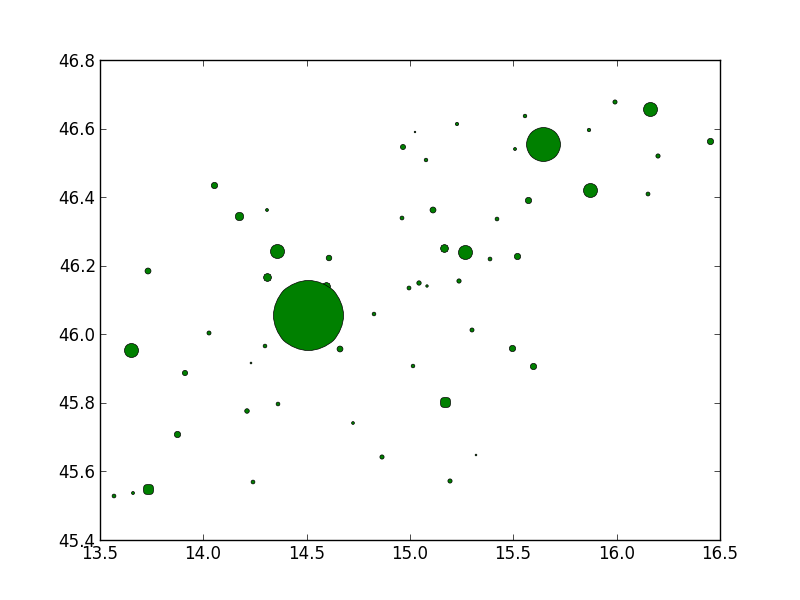
\includegraphics[scale=0.5]{../results/65/prebivalstvo_1998H1.png}
\end{frame} 

\begin{frame}
	\frametitle{Animation}
	\framesubtitle{Proportion of citizen over 65 years}
	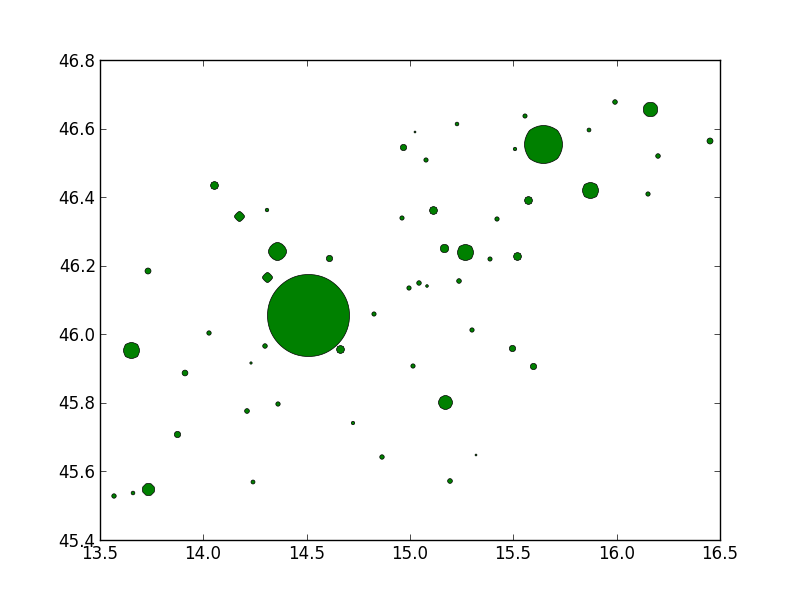
\includegraphics[scale=0.5]{../results/65/prebivalstvo_2004H1.png}
\end{frame} 

\begin{frame}
	\frametitle{Animation}
	\framesubtitle{Proportion of citizen over 65 years}
	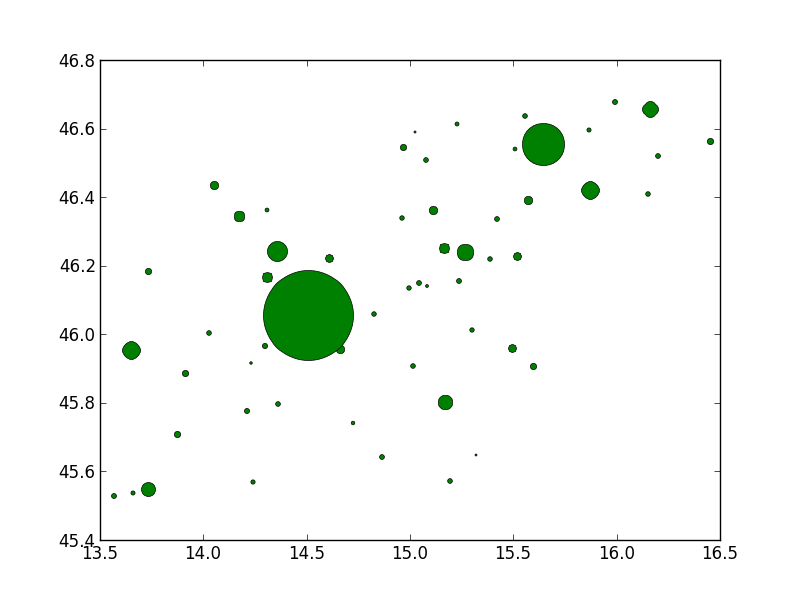
\includegraphics[scale=0.5]{../results/65/prebivalstvo_2008H1.png}
\end{frame} 

\begin{frame}
	\frametitle{Disances between time series}
	\begin{enumerate}
		\item Euclidean distance
		\item Dynamic time warping
	\end{enumerate}
\end{frame} 


\begin{frame}
	\frametitle{Euclidean distance}
	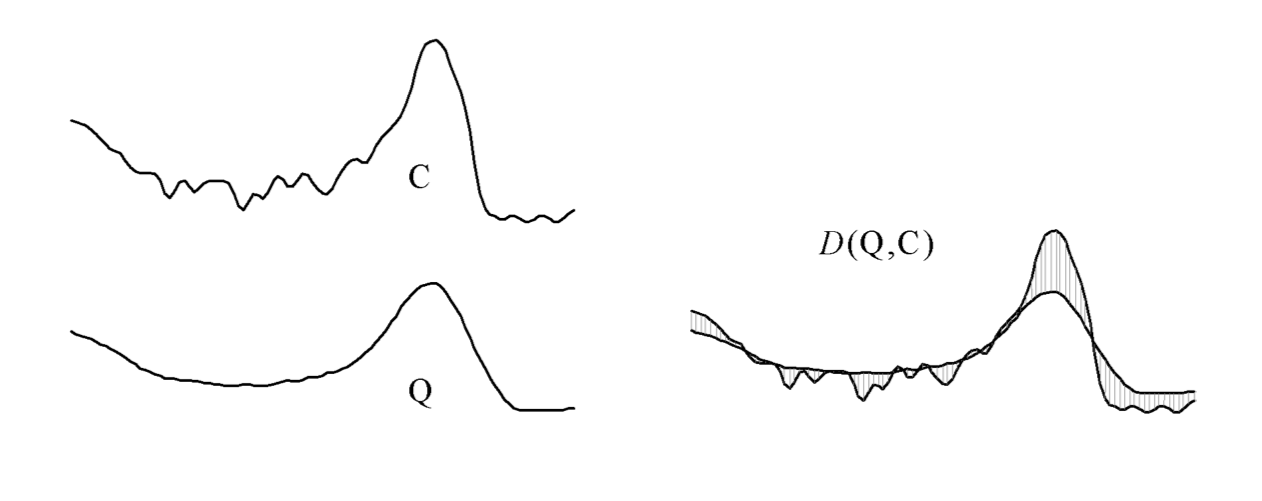
\includegraphics[scale=0.25]{../img/euclidean.png}
\end{frame} 

\begin{frame}
	\frametitle{Euclidean distance}
	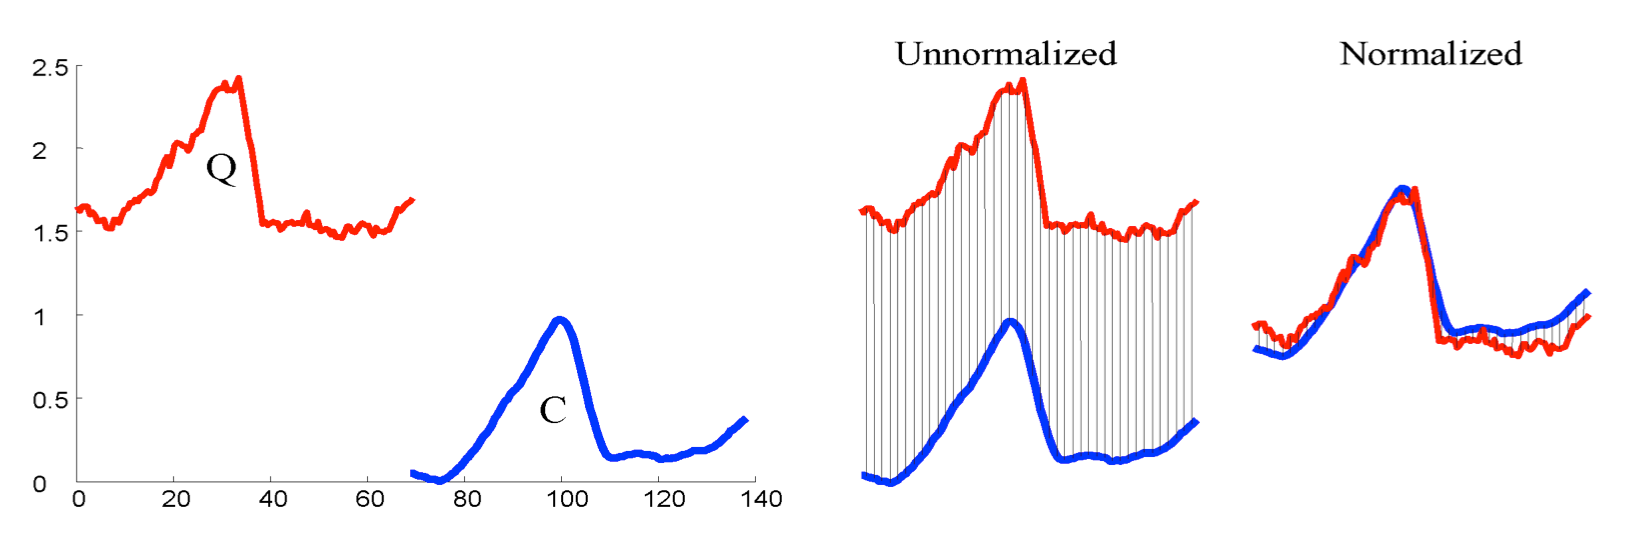
\includegraphics[scale=0.19]{../img/normalization.png}
\end{frame} 

\begin{frame}
	\frametitle{Dynamic Time Warp}
	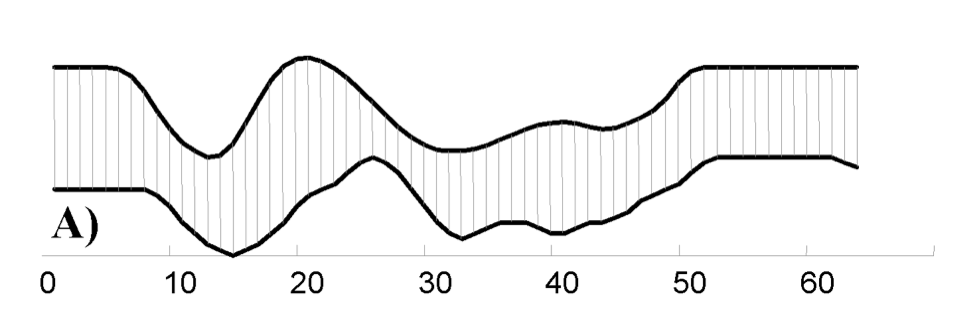
\includegraphics[scale=0.25]{../img/DTW.png}
\end{frame} 

\begin{frame}
	\frametitle{Dynamic Time Warp}
	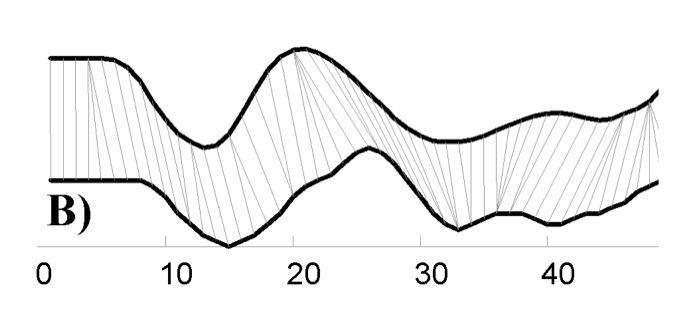
\includegraphics[scale=0.30]{../img/DTW2.png}
\end{frame} 

\begin{frame}
	\frametitle{Today's plan}.
	\begin{enumerate}
		\item Calculate distances between all Slovenian regions using DTW. 
		\item Perform hierarchical clustering on obtained distances. Are the results meaningful?
	\end{enumerate}
\end{frame}


\begin{frame}
	\frametitle{Distances between cities}
	
('Zagorje ob Savi', 'Cerknica') 278.0  \\
('Cerknica', 'Zagorje ob Savi') 278.0 \\
('Trbovlje', 'Ribnica') 313.0 \\
('Ribnica', 'Trbovlje') 313.0 \\
('Zagorje ob Savi', 'Tolmin') 315.0 \\ 
('Tolmin', 'Zagorje ob Savi') 315.0 \\
('Cerknica', 'Kocevje') 338.0 \\
('Kocevje', 'Cerknica') 338.0 \\
('Zagorje ob Savi', 'Kocevje') 365.0\\ 
... \\ 

\end{frame} 

\begin{frame}
	\frametitle{Distances between cities}
	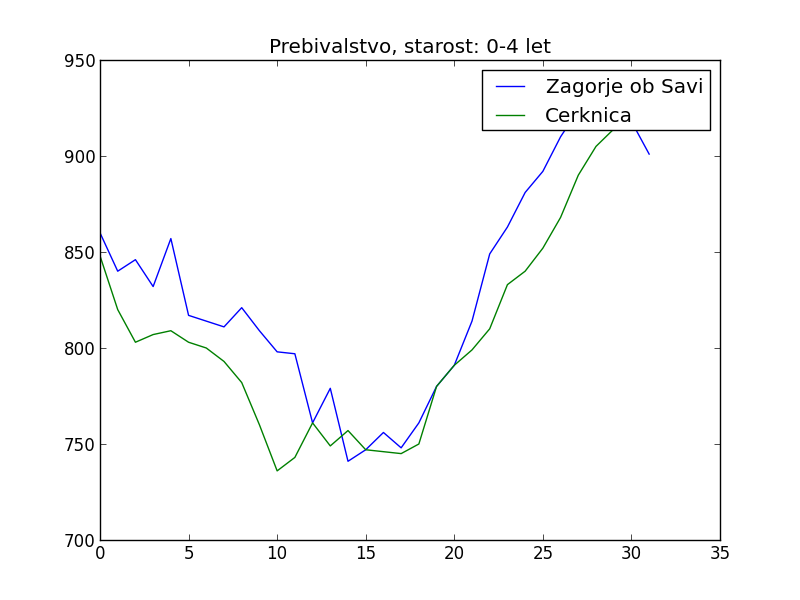
\includegraphics[scale=0.50]{../results/primerjava_0-4_let.png}
\end{frame} 

\begin{frame}
	\frametitle{Distances between cities}
	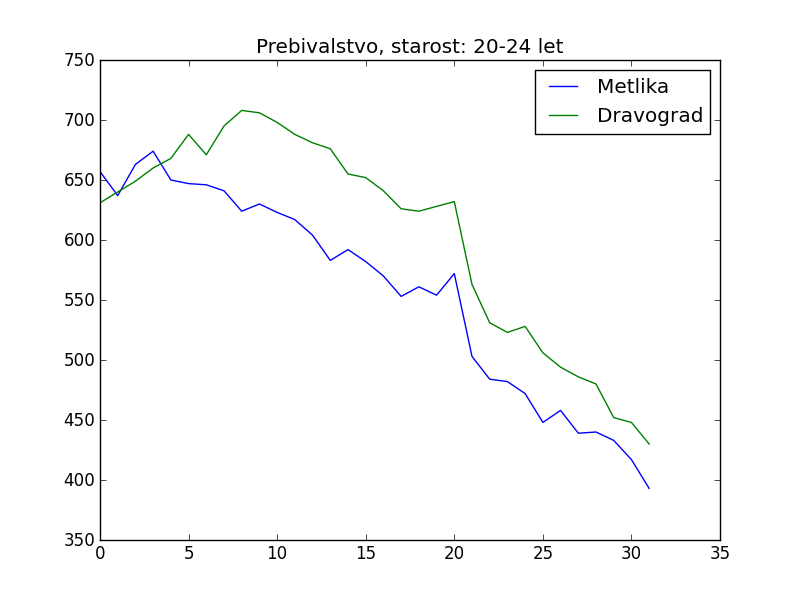
\includegraphics[scale=0.50]{../results/primerjava_20-24_let.png}
\end{frame} 

\begin{frame}
	\frametitle{Today's plan}.
	\begin{enumerate}
		\item Plot the data of Slovenian population as a stack plot.
		\item Explore emigration patterns of Slovenian Citizens over time. 
		\item How does the number of weddings in Slovenian regions change over time?
		\item How does the popularity of movies change with time? How does the popularity of genres overall change over time?	
	\end{enumerate}
	
\end{frame} 

\begin{frame}
	\frametitle{Data sources}.
	\begin{itemize}
		\item Statistični urad RS: http://pxweb.stat.si/pxweb/Dialog/statfile2.asp
		\item US National Accounts: http://unstats.un.org/unsd/snaama/dnllist.asp
	\end{itemize}
	
\end{frame} 
 
 
% etc
\end{document}
